\subsection*{Problema 14}

\textbf{Enunciado:} Calcular la integral:
\begin{align*}
\int \dfrac{5x + 4}{\sqrt{x^2 + 2x + 5}} \, dx
\end{align*}

\textbf{Solución:} 
Primero, relacionamos la derivada del radicando $u = x^2 + 2x + 5$, cuya derivada es $du = (2x + 2) \, dx$. 

Expresamos el numerador en función de esta derivada según las indicaciones:
\begin{align*}
5x + 4 &= \dfrac{5}{2}(2x + 2) - 5 + 4 \\
&= \dfrac{5}{2}(2x + 2) - 1
\end{align*}

Sustituimos esto en la integral original y separamos en dos integrales:
\begin{align*}
I &= \int \dfrac{\frac{5}{2}(2x + 2) - 1}{\sqrt{x^2 + 2x + 5}} \, dx \\
I &= \dfrac{5}{2} \int \dfrac{2x + 2}{\sqrt{x^2 + 2x + 5}} \, dx \\
&\quad - \int \dfrac{1}{\sqrt{x^2 + 2x + 5}} \, dx
\end{align*}

Para la primera integral ($I_1$), usamos la sustitución $u = x^2 + 2x + 5$:
\begin{align*}
I_1 &= \dfrac{5}{2} \int u^{-1/2} \, du \\
&= \dfrac{5}{2} \left( 2u^{1/2} \right) = 5\sqrt{x^2 + 2x + 5}
\end{align*}

Para la segunda integral ($I_2$), completamos cuadrados en el denominador:
\begin{align*}
x^2 + 2x + 5 &= (x + 2x + 1) + 4 \\
&= (x + 1)^2 + 2^2
\end{align*}

Aplicando la fórmula de integración directa:
\begin{align*}
I_2 &= \int \dfrac{dx}{\sqrt{(x+1)^2 + 2^2}} \\
&= \ln\left| (x+1) + \sqrt{x^2 + 2x + 5} \right|
\end{align*}

Combinando ambos resultados y agregando la constante de integración $C$:
\begin{align*}
I &= 5\sqrt{x^2 + 2x + 5} \\
&\quad - \ln\left| x + 1 + \sqrt{x^2 + 2x + 5} \right| + C
\end{align*}

\begin{figure}[H]
	\centering
	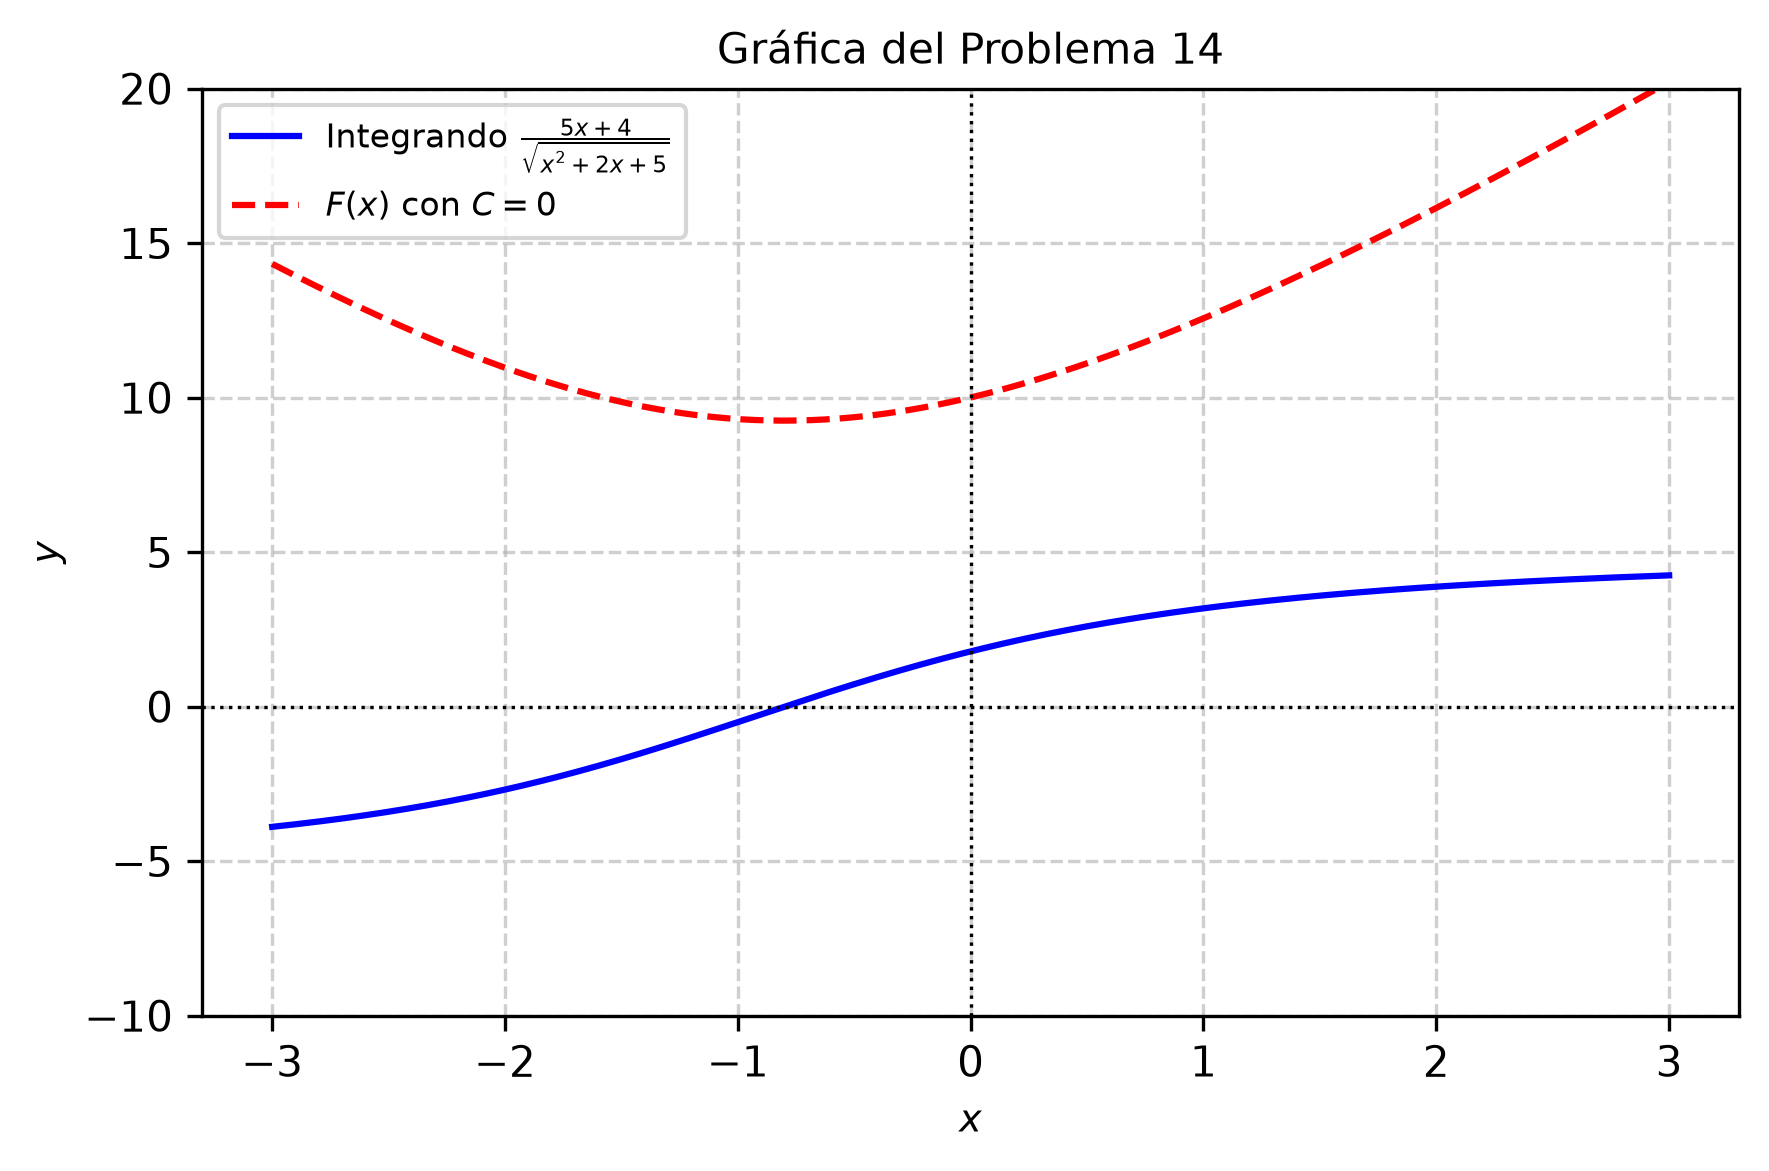
\includegraphics[width=\columnwidth]{semana_05/graficas/SEM05_P14_grafica.png}
	\caption{Representación gráfica de $f(x)$ y su antiderivada $F(x)$ evaluada para la constante de integración $C = 0$ (Problema 14).}
	\label{fig:problema14}
\end{figure}
